\documentclass[10pt, a5paper]{article}
\usepackage{pdfpages}
\usepackage{parallel}
\usepackage[T2A]{fontenc}
\usepackage{ucs}
\usepackage[utf8x]{inputenc}
\usepackage[polish,english,russian]{babel}
\usepackage{hyperref}
\usepackage{rotating}
\usepackage[inner=2cm,top=1.8cm,outer=2cm,bottom=2.3cm,nohead]{geometry}
\usepackage{listings}
\usepackage{graphicx}
\usepackage{wrapfig}
\usepackage{longtable}
\usepackage{indentfirst}
\usepackage{array}
\newcolumntype{P}[1]{>{\raggedright\arraybackslash}p{#1}}
\frenchspacing
\usepackage{fixltx2e} %text sub- and superscripts
\usepackage{icomma} % коскі ў матэматычным рэжыме
\PreloadUnicodePage{4}

\newcommand{\longpage}{\enlargethispage{\baselineskip}}
\newcommand{\shortpage}{\enlargethispage{-\baselineskip}}

\def\switchlang#1{\expandafter\csname switchlang#1\endcsname}
\def\switchlangbe{
\let\saverefname=\refname%
\def\refname{Літаратура}%
\def\figurename{Іл.}%
}
\def\switchlangen{
\let\saverefname=\refname%
\def\refname{References}%
\def\figurename{Fig.}%
}
\def\switchlangru{
\let\saverefname=\refname%
\let\savefigurename=\figurename%
\def\refname{Литература}%
\def\figurename{Рис.}%
}

\hyphenation{admi-ni-stra-tive}
\hyphenation{ex-pe-ri-ence}
\hyphenation{fle-xi-bi-li-ty}
\hyphenation{Py-thon}
\hyphenation{ma-the-ma-ti-cal}
\hyphenation{re-ported}
\hyphenation{imp-le-menta-tions}
\hyphenation{pro-vides}
\hyphenation{en-gi-neering}
\hyphenation{com-pa-ti-bi-li-ty}
\hyphenation{im-pos-sible}
\hyphenation{desk-top}
\hyphenation{elec-tro-nic}
\hyphenation{com-pa-ny}
\hyphenation{de-ve-lop-ment}
\hyphenation{de-ve-loping}
\hyphenation{de-ve-lop}
\hyphenation{da-ta-ba-se}
\hyphenation{plat-forms}
\hyphenation{or-ga-ni-za-tion}
\hyphenation{pro-gramming}
\hyphenation{in-stru-ments}
\hyphenation{Li-nux}
\hyphenation{sour-ce}
\hyphenation{en-vi-ron-ment}
\hyphenation{Te-le-pathy}
\hyphenation{Li-nux-ov-ka}
\hyphenation{Open-BSD}
\hyphenation{Free-BSD}
\hyphenation{men-ti-on-ed}
\hyphenation{app-li-ca-tion}

\def\progref!#1!{\texttt{#1}}
\renewcommand{\arraystretch}{2} %Іначай формулы ў матрыцы зліпаюцца з лініямі
\usepackage{array}

\def\interview #1 (#2), #3, #4, #5\par{

\section[#1, #3, #4]{#1 -- #3, #4}
\def\qname{LVEE}
\def\aname{#1}
\def\q ##1\par{{\noindent \bf \qname: ##1 }\par}
\def\a{{\noindent \bf \aname: } \def\qname{L}\def\aname{#2}}
}

\def\interview* #1 (#2), #3, #4, #5\par{

\section*{#1\\{\small\rm #3, #4. #5}}

\def\qname{LVEE}
\def\aname{#1}
\def\q ##1\par{{\noindent \bf \qname: ##1 }\par}
\def\a{{\noindent \bf \aname: } \def\qname{L}\def\aname{#2}}
}

\begin{document}
\title{Coreboot. Практическое знакомство со свободной альтернативой BIOS}
\author{Николай Стомчик, Минск, Беларусь\footnote{\url{mn3m00@gmail.com}, \url{http://lvee.org/en/abstracts/160}}}
\maketitle
\begin{abstract}
In modern Open Source world we need an open alternative to the proprietary product called BIOS. This alternative exists and is called coreboot. Coreboot is not fully equal to BIOS, it's only does initialization of RAM, execution of binary vendor blobs and starting some payload. The report main task is to cover how to start using it.
\end{abstract}
\subsection*{Введение}

Для построения полностью свободного стека ПО необходимо иметь свободную альтернативу проприетарным прошивкам \linebreak(firmware): классическому BIOS, либо UEFI в более новых системах. Такая альтернатива есть, и она называется coreboot.

Практические причины для использования CoreBoot \cite{bib1} могут быть:

\begin{itemize}
  \item Нужда в свободной альтернативе UEFI;
  \item Создание единого командно"=интерфейсного слоя в уровне \linebreak <<прошивки>> для кластерных решений на различных системах и архитектурах;
  \item Ускорить загрузку системы до ОС (до $\sim$~3~с)
  \item Разместить всю ОС (GNU/Linux, FreeBSD или другую) во flash"=памяти, позволив работать в режиме восстановления либо в полноценном режиме без использования жесткого диска;
  \item Общеобразовательные :)
  \item Предотвращение угрозы полумифического BadBIOS \cite{bib2, bib3};
\end{itemize}

\subsection*{Процесс загрузки Coreboot}

В процессе загрузки, устройство с coreboot проходит через следующие стадии:

\begin{figure}[h!]
  \centering
  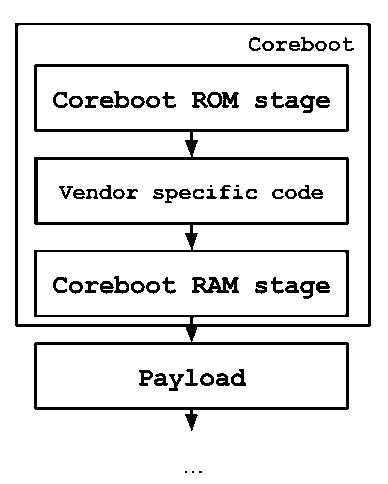
\includegraphics[scale=0.4]{10_2015_fig1}
\end{figure}

\begin{itemize}
  \item ROM stage "--- инициализация памяти и начальная инициализация чипсета; помимо общей схемы действий эта часть по понятным причинам очень специфична для конкретного оборудования, и здесь в обязательном порядке присутствует выполнение некоторых частей бинарной прошивки, которая определена производителем как обязательная для инициализации RAM, CPU или других системных устройств;
  \item RAM stage "--- нумерация устройств, назначение ресурсов, создание таблицы ACPI, SMM handler;
  \item Payload "--- выполнение некой полезной нагрузки, которая в \linebreak свою очередь может быть неким приложением либо загрузить операционную систему.
\end{itemize}

Coreboot не является полной заменой BIOS, т.к. не содержит никакой активной части по выполнению <<полезных действий>>: эта часть вынесена в отдельный модуль, называемый <<payload>> (полезная нагрузка). Достоинство такого разделения "--- возможность менять payload. Например, автором в качестве payload использован SeaBIOS, но есть альтернативы, такие как <<GRUB2>>, <<OpenBIOS>>. Можно <<выполнить>> в качестве payload ядро Linux или FreeBSD, а можно создать собственный: например, очень нужный в реальной практике payload, который пишет <<hello world>> и завершается:
\begin{verbatim}
 include <libpayload.h>
 int main(void)
 {
     printf("Hello, world from CoreBoot! :)\n");
     return 0;
 }
\end{verbatim}
Сборка этого шедевра функциональности может быть выполнена следующим способом:

\verb! $ lpgcc -o hello.elf hello.c!

После чего, данный Payload необходимо добавить в Ваш бинарный файл Coreboot.rom и можно перейти на этап загрузки его в ПЗУ.

\subsection*{Подготовка coreboot к прошивке}

По понятным причинам поддержка всего многообразия чипсетов и материнских плат проектом coreboot оставляет желать лучшего. Однако, если ваше оборудование попало в число поддерживаемых, процедура перепрограммирования может оказаться не самая простая, особенно в случае если производитель ноутбука либо компьютера поспешил обезопасить себя от желающих самостоятельно заменить базовую микро"=программу.

В частности, подготовительные шаги для установки coreboot на основе личного опыта автора по перепрошивке ThinkPad x201\cite {bib4} выглядели следующим образом:

\begin{itemize}
  \item тщательное изучение документации по разборке ноутбука, чтобы отыскать чипы памяти BIOS и CMOS;
  \item чтение datasheet'ов на ROM и выяснение специфики его программирования;
  \item покупка (либо сборка) программатора и разъёмов (SOIC"=8P) для ISP программирования;
  \item извлечение videorom.bin из оригинального проприетарного \linebreak BIOS, которую можно получить из ОЗУ в процессе работы системы;
  \item создание резервной копии firmware с помощью программного или аппаратного программатора (эксперименты с подобными материями быстро излечивают от неоправданного оптимизма);
  \item клонирование coreboot и его зависимостей из git, выполнение `make menuconfig' и `make', с последующими \emph{n} часами сборки с удовлетворением всех зависимостей;
  \item программирование в ПЗУ результирующего бинарного файла;
  \item многочасовое тестирование компьютера с новой микропро\-граммой, с использованием нагрузочных тестов и проверкой всего оборудования.
\end{itemize}

\begin{figure}[h!]
  \centering
  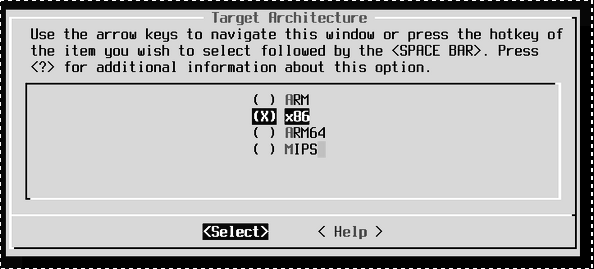
\includegraphics[scale=0.4]{10_2015_fig2}
\end{figure}

Саму запись микропрограммы в постоянную память можно выполнить из Linux её штатными средствами "--- <<flashrom>>, либо, если этот этап завершился неудачей "--- аппаратным программатором.  В случае с Thinkpad x201 для программирования MX25L6445E (8MB Serial Flash) подходят программаторы:

\begin{itemize}
  \item BusPirate v4;
  \item minipro TL866C;
  \item Raspberry PI;
  \item любой другой, который умеет программировать через SPI.
\end{itemize}

Из"=за того, что программная перепрошивка оказалась заблокирована вендором (а способ разблокировки, применяемый для обновления фирменной прошивки, на данный момент неизвестен), для LENOVO Thinkpad x201 пришлось воспользоваться аппаратным программатором minipro TL866. При работе из GNU/Linux команда перепрошивки должна выглядеть примерно следующим образом:

\begin{verbatim}./minipro -i -p "MX25L6445E @SOP8" -w {Patch_for_your_
coreboot}build/coreboot.rom\end{verbatim}

\begin{figure}[h!]
  \centering
  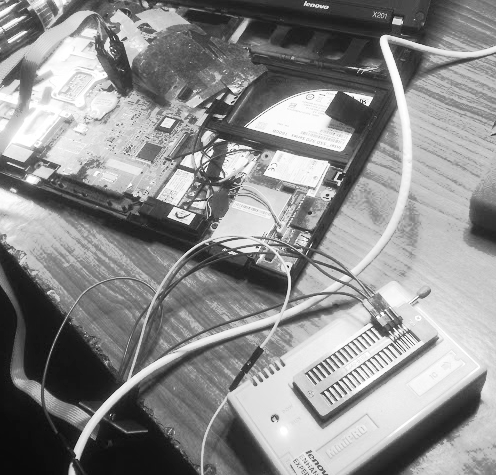
\includegraphics[scale=0.4]{10_2015_fig3}
\end{figure}

\subsection*{Советы по внутрисхемному программированию}

\begin{itemize}
  \item Важно следить за уровнем питания микросхемы на плате. Если питания не достаточно, есть смысл воспользоваться внешним блоком питания. Обычный стандартный блок ATX для таких задач вполне подходит (необходимо +3.3V);
  \item Для получения корректных результатов считывания и записи <<Земля>> (GND) программатора, корпуса ноутбука и блока питания должны быть соединены;
  \item Перед записью будет не лишним попробовать прочитать содержимое микросхемы N раз и проверить контрольные суммы "--- SHA или MD5. Если они не совпадают, проблема наверняка кроется в двух предыдущих пунктах.
\end{itemize}

\subsection*{Работоспособность после прошивки}

В результате экспериментов с ThinkPad x201 были выявлены следующие мелкие баги (которые, возможно, на момент чтения этой статьи уже будут исправлены):

\begin{itemize}
  \item ограничение <<на перегрев CPU>> теперь отсутствует, что требует добавить ещё один скрипт проверки на перегрев, либо понизить немного частоту CPU до стабильной, что бы этот перегрев и не возникал;
  \item каждые 10 минут возникает <<засыпание>> экрана, вне зависимости от установок xset (Исправляется \verb!xset -dpms off!);
  \item при подключенном втором дисплее перестает регулироваться яркость подсветки основного дисплея используя горячие клавиши;
  \item понадобилось переписать скрипт регулировавший частоту процессора из"=за новых значений шага для частоты CPU;
  \item проигрывание звука на колонках отключается программно, то есть при включенных наушниках можно включить воспроизведение на встроенных динамиках ноутбука;
\end{itemize}

Однако список работающего функционала оказался внушительным:

\begin{itemize}
  \item 3G GPRS modem;
  \item 4G+4G RAM;
  \item функциональные клавиши ThinkPad (фонарик, громкость);
  \item расширения VT"=x процессора;
  \item аппаратная поддержка AES в CPU;
  \item WIFI;
  \item Ethernet;
  \item Все порты ноутбука (USB, DP, HDMI, DSUB), а также док"=станция;
  \item Устройство считывания отпечатков пальцев;
  \item Управление питанием устройства, контроль за состоянием батареи.
\end{itemize}

Время загрузки микропрограммы, инициализации всего аппаратного обеспечения и передача управления начальному загрузчику ОС (GRUB2) сократилось с $\sim$ 50 с до $\sim$ 4 с, и при том большую часть из этого времени SeaBIOS ожидает нажатия F12 для выбора устройства загрузки. Хотя ускорение загрузки не являлось целью данной работы, нельзя не отметить, что логотип coreboot соответствует его значению:

\begin{figure}[h!]
  \centering
  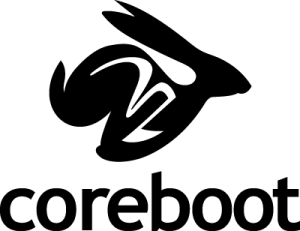
\includegraphics[scale=0.3]{10_2015_fig4}
\end{figure}

Конечно, данное обстоятельно не может не радовать.

\subsection*{Отладка}

Подготовленный payload можно протестировать в эмуляторе \linebreak QEMU"=KVM перед запуском, чтобы удостовериться, что всё работает как требуется. В самом же устройстве можно использовать традиционный для этих задач индикатор POST"=кодов, отображающий значения, отправленные в порт 80h, последовательный порт "--- либо PC"=speaker как средства диагностики состояния и процесса загрузки.

\begin{figure}[h!]
  \centering
  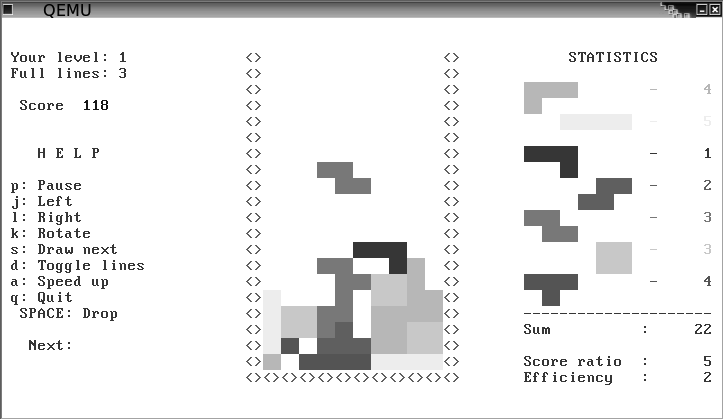
\includegraphics[scale=0.55]{10_2015_fig5}
\end{figure}


\begin{thebibliography}{9}
\bibitem{bib1} {\href{http://www.coreboot.org/}{http://www.coreboot.org}}
\bibitem{bib2} {Bruce Schneier. badBIOS // Schneier on Security. \href{https://www.schneier.com/blog/archives/2013/11/badbios.html}{https://www.schneier.com/blog/archives/2013/11/badbios.html}}
\bibitem{bib3} {Jonathan Brossard. Hardware backdooring is practica. // DEFCON 20 presentation. \href{http://www.slideshare.net/endrazine/defcon-hardware-backdooring-is-practical}{http://www.slideshare.net/endrazine/defcon-hardware-backdooring-is-practical}}
\bibitem{bib4} {\href{https://github.com/mn3m0nic/ffts/blob/master/thinkpad.md}{github.com/mn3m0nic/ffts/blob/master/thinkpad.md}}\end{thebibliography}
\end{document}
